\documentclass{article}

\usepackage{graphicx}
\usepackage{hyperref}

\title{Semi-automatic SuperCon staging area for ingesting structured data collected from scientific literature}
\author{Authors}

\begin{document}

\maketitle

\begin{abstract}
    TBA
\end{abstract}

\section{Introduction}
The publication rate in scientific publications is growing at a significant rate across various fields with an exponential trend in materials science~\cite{Pratheepan_2019}. 
The adoption of new statistical methodologies for materials informatics (MI) using data-driven research has stressed the needs of large structured materials information to support data-driven research. 
In materials science, however, it is still a common practice to extract data manually from scientific articles, like in the Pauling File~\cite{Blokhin2018ThePF_paulingFile}, AFLOW~\cite{aflowcurtarolo2012aflow} databases for example. 
Large aggregated databases created more recently, such as the Material Project~\cite{materialsprojectJain2013}, combine human validation with automatic processes to produce initial predictions and gather materials data. 

[DFT / calculated data is more popular. - Experimental extracted data is less used]

At first glance, it may seem more straightforward to create a single manual procedure that can extract information from diverse sources like plots, tables, and text all at once. However, while this approach may be viable in the short term, its sustainability diminishes over time. 
On the other hand, constructing an automated process to accomplish this task presents many challenges. In case of scientific publications, plots, tables and text necessitates different treatments, and the resulting outputs must be merged and verified manually. Despite the challenges, it is possible to transition gradually towards automation by implementing iterative steps. This iterative approach involves reducing human involvement progressively while simultaneously optimising the efficiency of required human actions. 

In superconductors research, the gold standard database is SuperCon~\cite{SuperCon}, which was built manually over more than a decades from the National Institute for Materials Science (NIMS). 
Despite being praised for its excellent quality in numerous reports~\cite{roter2020predicting, stanev_machine_2017, tran2022machine, konno2021deep}, the updates of SuperCon have become increasingly challenging due to the high publication rate. However, in response to the need for a more efficient approach to sustain productivity, we embarked on the development of an automated system for extracting material and property information from text contained in relevant scientific publications~\cite{doi:10.1080/27660400.2022.2153633}. This automated process enabled the rapid creation of SuperCon2, a comprehensive database of superconductors containing over 35,000 entries, accomplished in just a few days. 

Ensure the same quality as SuperCon while automating the extraction of structured superconductors data poses significant challenges. 
We developed a web interface designed to facilitate the curation process, involving the active and ongoing management of data through its lifecycle of interest, specifically tailored for our superconductors database but open to potential adaptation other data structures. 
Our interface aims to maintain quality, add value, and provide for re-use over time, while making the curation process faster, more effective, and user-friendly.

There are several tools for data annotation, such as Inception~\cite{klie-etal-2018-inception}, Doccano~\cite{doccano}, at the moment of writing this article, we are not aware of any other curation tools for materials extracted databases. 
This paper introduces our curation tool, SuperCon2, which serves as a data staging area towards SuperCon. The tool allows for the visualisation, correction, and integration of automatically extracted data into the SuperCon database, while triggering a feedback loop to improve the machine learning (ML) models.

Our contributions in this work are as follows:
\begin{itemize}
    \item We designed a efficient scalable ingestion process for process batches of PDF documents,
    \item We designed a set of anomaly detection scripts ....
    \item We present a new interface specifically designed for data curation in materials science, 
    \item We integrate the visualisation of the extracted materials-related entities with the PDF document viewer. This utilises coordinates extracted by Grobid~\cite{GROBID} and it was demonstrated in other fields by~\cite{wang2022hammer}. [Add more references] 
    \item We establish a feedback loop mechanism that generates training data at the sentence level based on the data correction process.
\end{itemize}

The subsequent sections of this paper elaborate on the interface and its design principles, the ingestion and corrections processes. Finally, we present some results from the feedback loop. 

\section{User interface}

The SuperCon2 curation interface offers several key features to facilitate the data curation process.

It provides a comprehensive view that visualises materials and their related properties as a table which includes search, filtering, and sorting functionality (Figure~\ref{fig:curation-interface-database}). 
The schema consists of two main classes: material information (material names, formulas, shape, etc.) and properties (T\textsubscript{c}, applied pressure, measurement method, etc.). The complete list including examples is reported in our previous work~\cite{lfoppiano2023automatic}.

\begin{figure}[t]
  \centering
  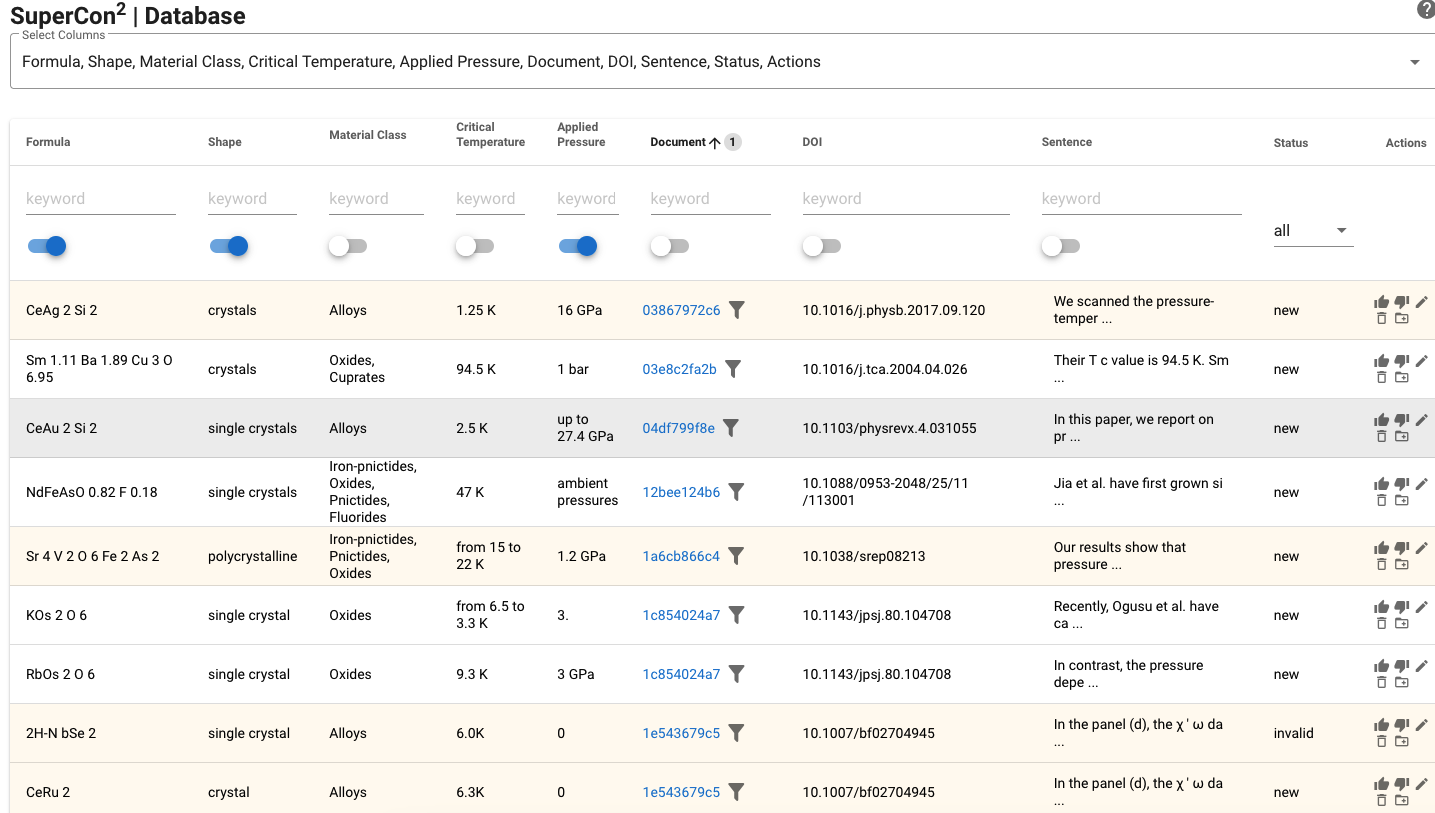
\includegraphics[width=1\textwidth]{images/supercon-curation-database} 
  \caption{Curation interface showing the database as a table}
  \label{fig:curation-interface-database}
\end{figure}


During the curation process is often necessary to navigate back and forth to the related section to the extracted record that is being examined. The curation interface provide a document viewer combining a table with the extracted records and the viewer of their respective document (Figure~\ref{fig:curation-interface-pdf-viewer}). The viewer highlights the annotations that identify materials and properties, enabling users to easily locate and reference the extracted information within the document.

Each record presented can be modified, removed, or flagged. The flagging was built with the idea of having two phases curation: in the first phase, the records are examined quickly mostly without checking the document information, and the users flags any record that judge incorrect. The second step, slower, the user goes through the invalid information and examine them thoughtfully correcting when needed and stepping back to the document to check the context. 

The interface automatically collects training data. When a record is corrected, the information pertaining to the sentence, spans (annotations), and tokens (including layout information, fonts, and other features) is gathered, enabling the generation of valuable training data for further improvements in the automated extraction process.

\begin{figure}
  \centering
  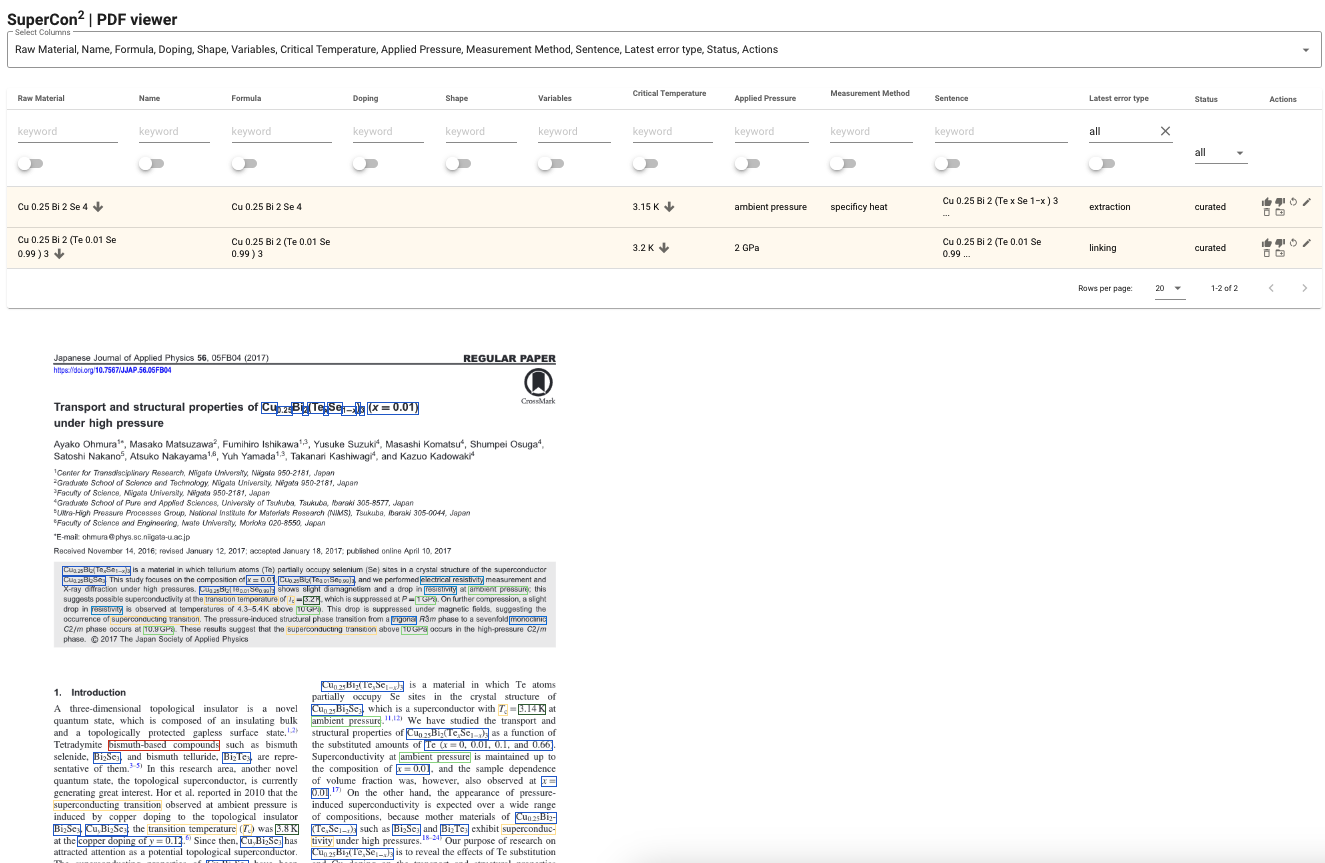
\includegraphics[width=1\textwidth]{images/supercon-curation-pdf-viewer} 
  \caption{PDF viewer. The page includes a table showcasing records extracted from the  current document, along with the PDF content and accompanying annotations.}
  \label{fig:curation-interface-pdf-viewer}
\end{figure}


\subsection{Data flow and model}
\label{subsec:data-flow}

The data flow is first introduced in our previous work~\cite{lfoppiano2023automatic} using a Map-Reduce approach. 
First, in the "extraction task", the PDF documents are stored and processed by grobid-superconductors which transforms them in the corresponding annotations format. The format is illustrated in Figure~\ref{fig:data-flow-2} and is structured as a list of "passages" (sentences or paragraphs). 

\begin{figure}[t]
  \centering
  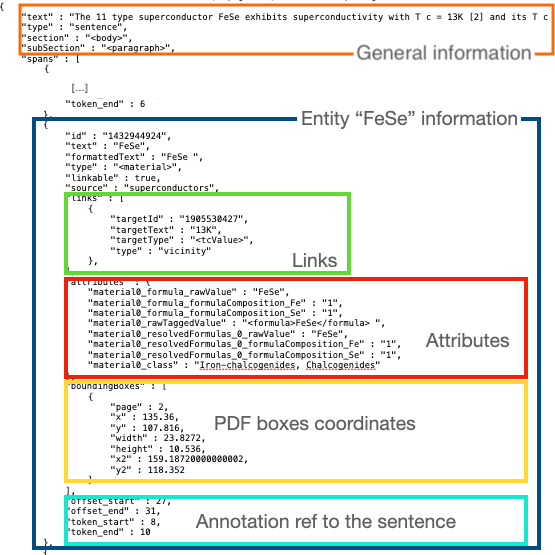
\includegraphics[width=0.8\textwidth]{images/data-flow-2} 
  \caption{Example of a passage extracted in the "extraction task". We highlight the different structured information in a single span: links, attributes, PDF coordinates (to visualise annotations on the PDF document), and annotations references within the sentence (to visualise annotations on text).}
  \label{fig:data-flow-2}
\end{figure}

Each passage is composed by the following attributes: the text of the passage, the type, of passage (sentence or paragraph), the main section: header, body, and annex and the subsections: title, abstract, paragraph, caption. 
Furthermore, there is the list of spans containing the extracted entities which include the text, type, attributes, the tokens containing layout information (font size, font face, superscript, subscript, bold, italic, coordinates), an unique identifier, and other internal information (source ML model) and whether is allowed to be linked (temperatures not classified as superconductors critical temperatures are set to linkable = False).
The attributes are stored as as a key-value and mainly contains information extracted by the material parser: the formula, the structured composition, the material class.  

Second, in the "aggregation task", the annotated documents are aggregated as flat table format, of which each row become a \textit{record} of one material and their properties. For materials containing more information, for example when the paper describes different doping ratio, the records are duplicated and the non-variable attributes are copied. 
% In Figure~\ref{fig:data-flow-3} there is an example of flat table record. 

% \begin{figure}
  % \centering
  % 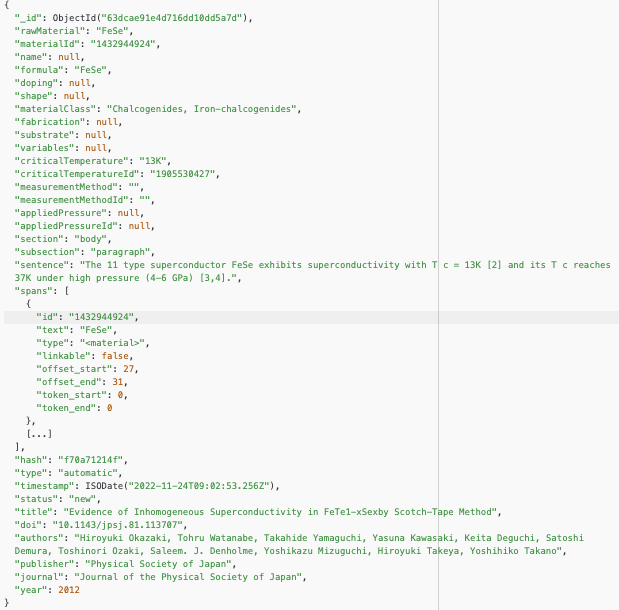
\includegraphics[width=0.8\textwidth]{images/data-flow-3} 
  % \caption{Example of record after the aggregation.)}
  % \label{fig:data-flow-3}
% \end{figure}

\subsection{Design principles}
\label{subsec:design-principles}

The design principle are a set of rules we chose at the beginning of the development. 

\paragraph{Blind correction}
This interface has been built without any multi-user mechanism. 
The data is allocated to different curators by generating randomised links to the application. Each link opens records extracted from a specific document. 
The justification for this approach is twofold: a) the allocation is totally random and each curation does not know any information about the others, and b) the multi-user implementation requires large effort without any particular scientific gain. 

\paragraph{Data duplication} When a record is modified its data is duplicated and a new record is created. 
This, allows us now to collect curation records knowing which data was corrected, when and how many changes were done. In future, this feature, will simplify the implementation of the undo/redo operations. 
When a record is deleted, his status is modified to "removed", and the record hidden. 

On the contrary, binary records, such as PDF documents, are not duplicated, for saving disk space. Obviously, this does not forbid to load two different PDF documents of the same article, because the hash code would be different. In such cases the anomaly detection (Section~\ref{subsec:anomaly-detection} will notice the duplication and report it. 

The PDF documents binary content is used to generate a hash code of 8 character which is used to avoid duplicated PDF document, for linking documents and records within the database. Each record, and even each span have its own unique identifier which are calculated using the span attributes.

\begin{figure}
  \centering
  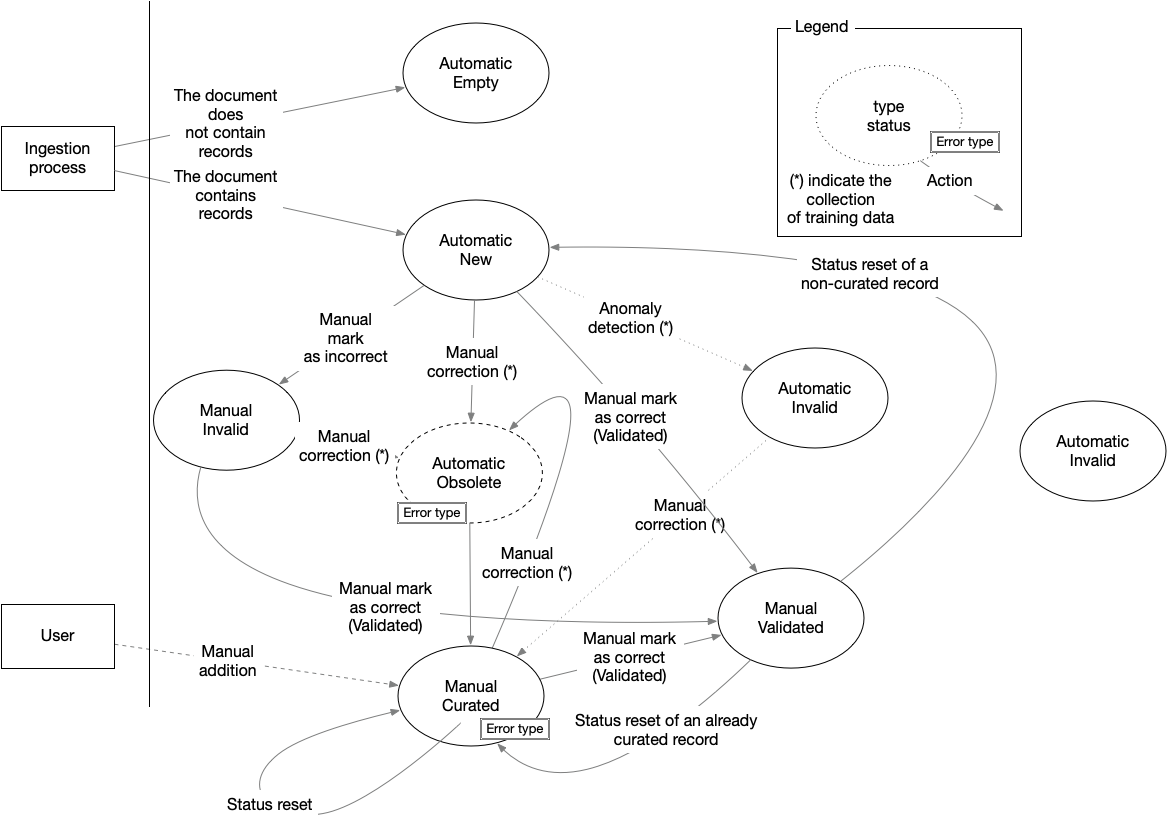
\includegraphics[width=1\textwidth]{images/record-correction} 
  \caption{Schema of the curation workflow. Each state is characterised of two properties: type and status, and one action, as indicated on the top right corner. "Error type" indicate the action of storing the error type for that specific action.}
  \label{fig:curation-workflow}
\end{figure}

\paragraph{Type and Status} Each \textit{record} has two workflow-related fields which are combined to identify the state of the workflow, which is illustrated in Figure~\ref{fig:curation-workflow}. 
The status indicate the record curation status from the data point of view, and is summarised in Table~\ref{tab:record-status}

\begin{table}[htbp]
\centering
\begin{tabular}{|p{2cm}|p{10cm}|}
\hline
\textbf{Status} & \textbf{Description} \\
\hline
new & Default status when a new record is created. \\
\hline
curated & The record has been updated by a human. \\
\hline
validated & The record was validated by a human. \\
\hline
invalid & The record is wrong or inappropriate for the situation (e.g., Tm or Tcurie extracted as superconducting critical temperature). \\
\hline
obsolete & Assigned to a record when it is modified, triggering the creation of a new record (internal status, not visible to users).\\
\hline
deleted & The record has been removed by a curator (internal status, not visible to users). \\
\hline
\end{tabular}
\caption{Record status definitions}
\label{tab:record-status}
\end{table}
    
The type indicates whether the record has been created or modified manually or automatically. The value "automatic" is provided when the data is loaded and/or when the anomaly detection perform some operations. All other cases it is flipped to "manual". 

\paragraph{Error types} Error types were first introduced in~\cite{lfoppiano2023automatic} while performing manually the the End 2 End evaluation. They were combined with the evaluation to provide more detailed information on the reasons why certain extracted values were not correct. 
Since such statistics demonstrated to be useful during the development, we have extended the scope to add additional values related to data curation and validation (Table~\ref{tab:error-types}).

\begin{table}[htbp]
\centering
\begin{tabular}{|p{4cm}|p{8cm}|}
\hline
\textbf{Name} & \textbf{Description} \\
\hline
From table & The entities Material $\rightarrow$ Tc $\rightarrow$ Pressure are identified in a table. At the moment, table extraction is not performed. \\
\hline
Extraction & The material, temperature, pressure are not extracted (no box) or extracted incorrectly. \\
\hline
Linking & The material is incorrectly linked to the Tc given that the entities are correctly recognized. \\
\hline
Tc classification & The temperature is not correctly classified as "superconductors critical temperature" (e.g., Curie temperature, Magnetic temperature...). \\
\hline
Composition resolution & The exact composition cannot be resolved (e.g., the stoichiometric values cannot be resolved). \\
\hline
Value resolution & The extracted formula contains variables that cannot be resolved, even after having read the paper. This includes when data is from tables. \\
\hline
Anomaly detection & The data is automatically modified by the anomaly detection script. \\
\hline
Curation amend & The curator is updating the data which does not present issues due to the automatic system. \\
\hline
\end{tabular}
\caption{Summary of error type values and description.}
\label{tab:error-types}
\end{table}

In the curation interface we made the error type mandatory at each modification, including deletion as well. Since often the modifications are not related to a mistake, e.g. adding a space in a formula to make it more clear, or replacing garbled characters, we allow an additional error type called "Curation amend" which indicate that the problem is not related to the automatic system. This covers also the case where the modification corrects a mistake from another curator. 
When the updated is made, a new record is created, and the error type is stored in the previous record. The workflow schema in Figure~\ref{fig:curation-workflow} indicate "error type" in the states that requires it's selection. 

\subsubsection{Usability}
What are our usability goals? 
What are the metrics for usability? 

[Mato]
PDF viewer jump from table to the related part of the PDF document, 

We implemented keyboard shortcuts, to allow people to move around without using the mouse 
[We might need an experiment to measure the improvement in efficiency]




\subsubsection{Curation and processing logs}

The Supercon\textsuperscript{2} interface records minimal information regarding the ingestion (processing log) and the curation process (curation log). 
The processing log is filled-up when the data is ingested, it was build to have minimal functions able to explain why certain documents haven't been processed (Figure~\ref{fig:processing-log}). 
Grobid was built focusing on speed and robustness, and contains several fail-safe mechanisms to avoid crashing the system when a document is either too big or does not contains valuable information, for example does not have any text. Old PDF documents (e.g. before 1990) are likely have been scanned and contains only images. 
Examples of too big documents are dissertation thesis with more than 100 pages, that might be collected by mistake. 


\begin{figure}
  \centering
  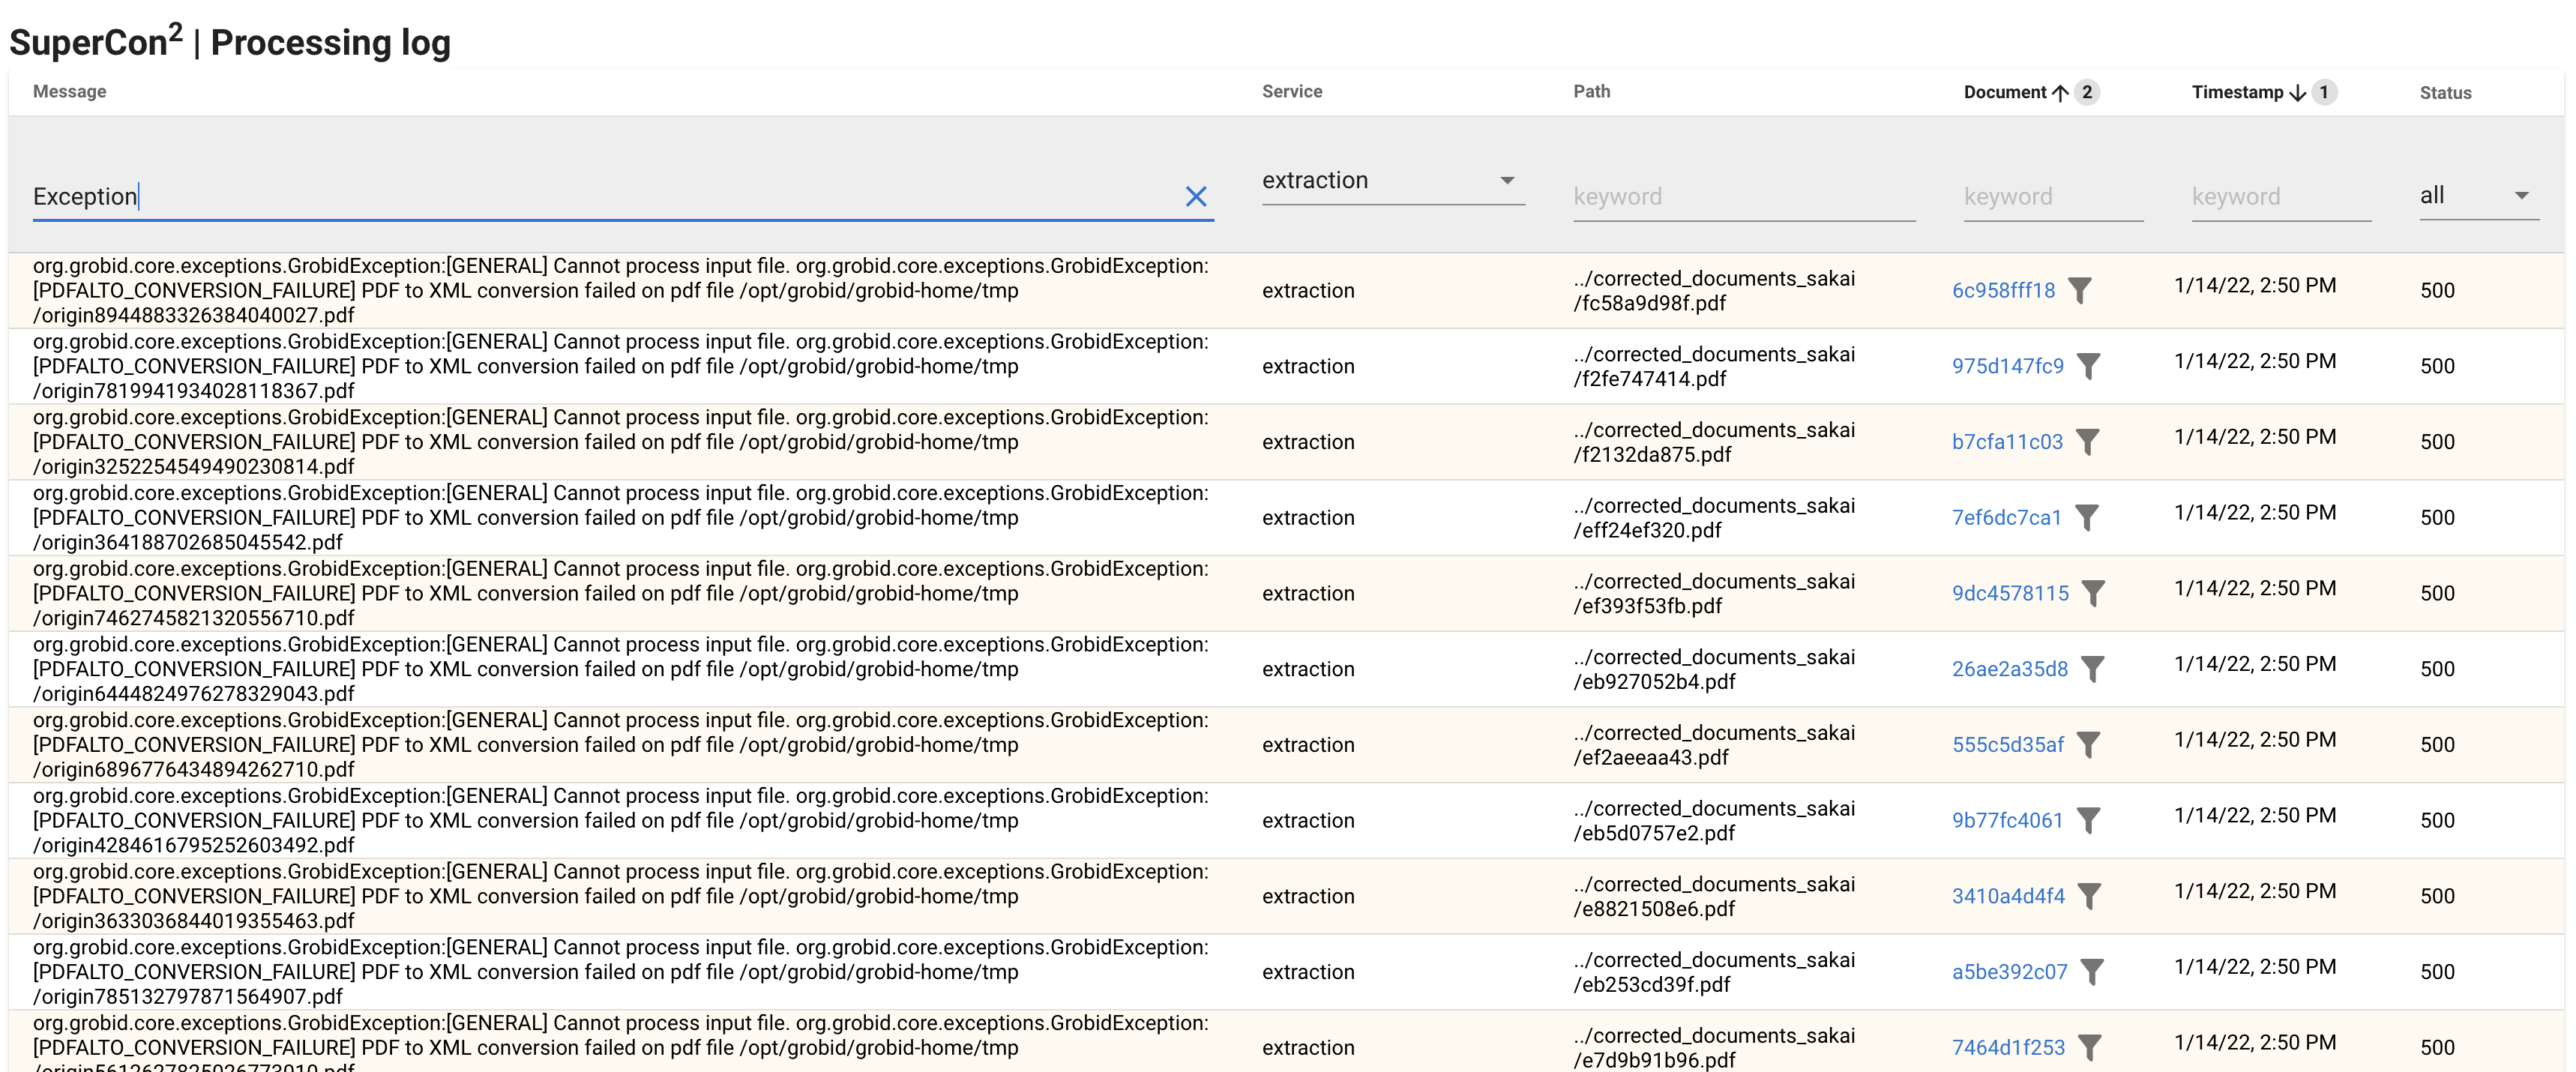
\includegraphics[width=1\textwidth]{images/processing-log.png} 
  \caption{Processing log, showing the result of each of the actions described in Section~\ref{subsec:data-flow}, and if an error has occurred}
  \label{fig:processing-log}
\end{figure}

The curation log provide a view on the corrections that are performed in an aggregated page. 
The curation log shows all the records that have been updated and when. It includes also the history of each record (Figure~\ref{fig:curation-log}).

\begin{figure}[t]
  \centering
  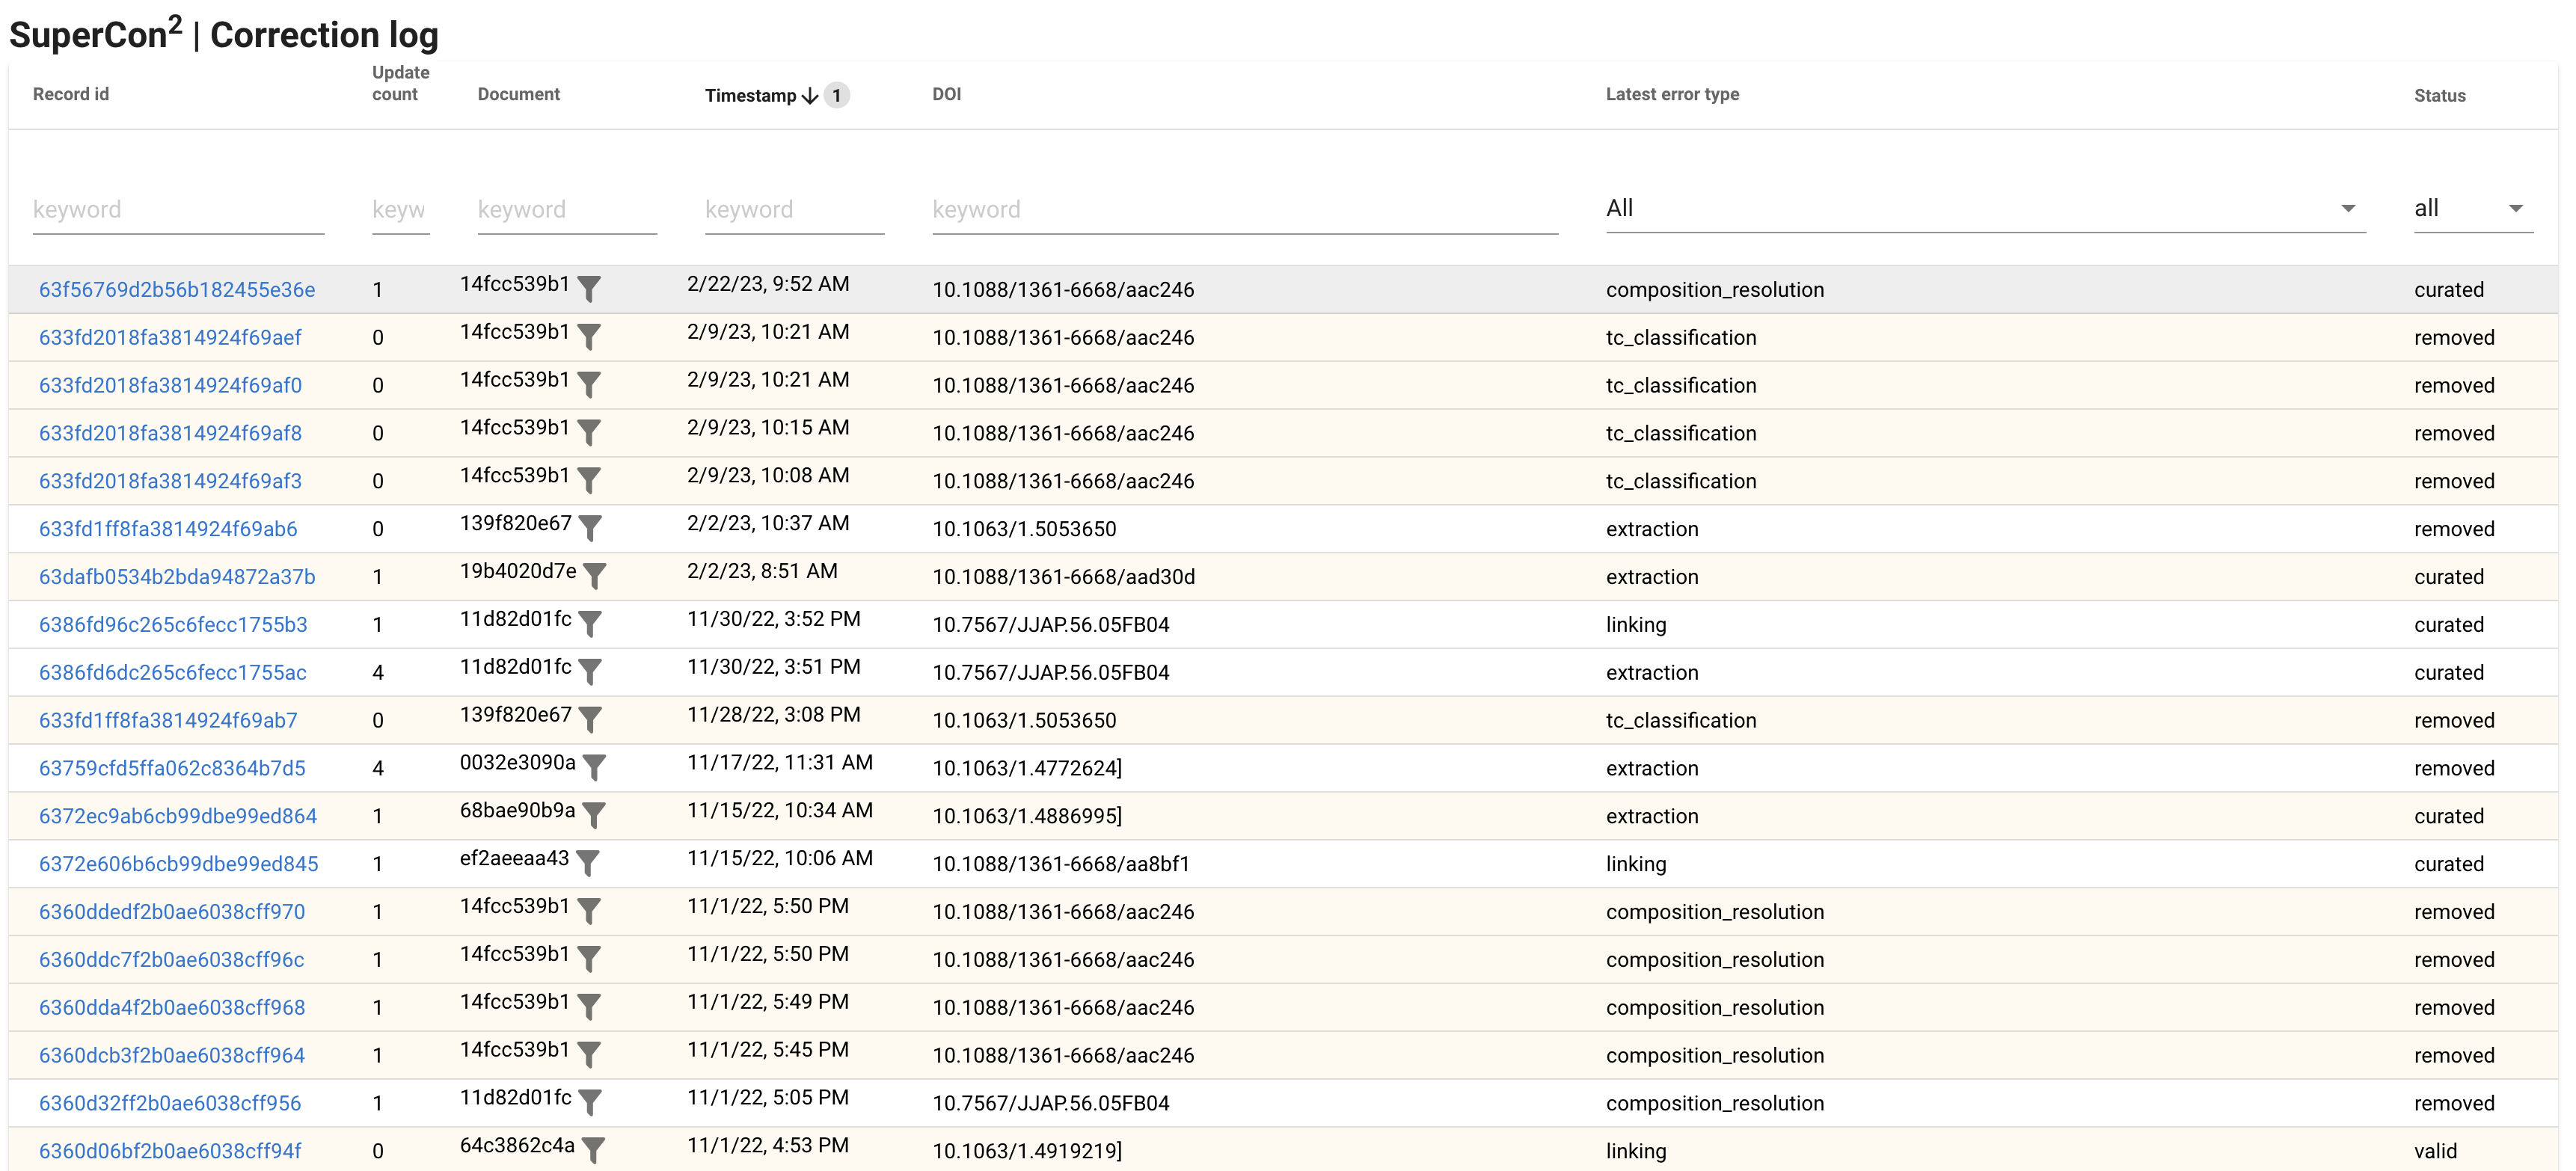
\includegraphics[width=1\textwidth]{images/curation-log} 
  \caption{Curation log, indicating each record, the number of updates, and the date/time of the last updates. }
  \label{fig:curation-log}
\end{figure}


\section{Data correction}

\subsection{Manual correction}
[Terashima/Sakai] Discussion about the guidelines (which should be published in a format other than Powerpoint)

\subsection{Anomaly detection}
\label{subsec:anomaly-detection}
Anomaly detection is the process of identifying unusual or unexpected events or patterns in data. In this project we limited the implementation to a simple rule-based filter that focuses on formulas and T\textsubscript{c} values.
When the filter identifies an anomaly, it sets the corresponding record status as "invalid" and its type as "automatic" which can be identified by curators. 
The rules include conditions such as marking invalid all the extracted T\textsubscript{c} greater than room temperature (273 K), or evaluating the validity of compounds formulas ensuring they can be parsed. 
It is crucial to stress that these rules are to be taken lightly and further validation by curators is necessary. Tc values above room temperature are perfectly legig in researchers' hypotheses or preliminary calculations. Stochiometric formulas with doping variables are still valid, even if they cannot be parsed properly. 
When the filter was applied to the SuperCon\textsuperscript{2} database, it found 70 records with invalid T\textsubscript{c} and 7000 records with invalid formulas. 

Two additional filters that can theoretically help increase simplify the work of curators are: 
\begin{itemize}
    \item Identification of duplicated documents wrongly loaded under different MD5 hashes, this could be performed by matching via bibliographic data (first by DOI, then by title and authors, etc), 
    \item perform the anomaly detection perpendicularly by aggregating each formula and verify the variation in the collected Tc. The variation can be compared with a tolerance of roughly 1 or 2 K. 
\end{itemize}

[TODO: write a simple script to test these two additional ideas and how many records they can identify]

\subsection{Feedback loop training data creation}

One of the key hidden features of this interface is the possibility to generate training data automatically, every time a record is corrected. 

The process works in the following way, when a correction is performed:
\begin{itemize}
    \item the new record with updated information is prepared and stored, 
    \item if the training data exists (e.g. another correction within the same sentence was already performed), then the process finishes
    \item using the record document identifier (the hash), the latest annotation document is retrieved
    \item using the record "materialId" the entity annotation is searched within the annotation document,
    \item when the material is found the passage object containing the text, spans, tokens and other information are collected and saved in a separate collection. The record id is also attached to the training data 
\end{itemize}

The training data can be inspected in a specific section (Figure~\ref{fig:training-data-view}).

\begin{figure}[t]
  \centering
  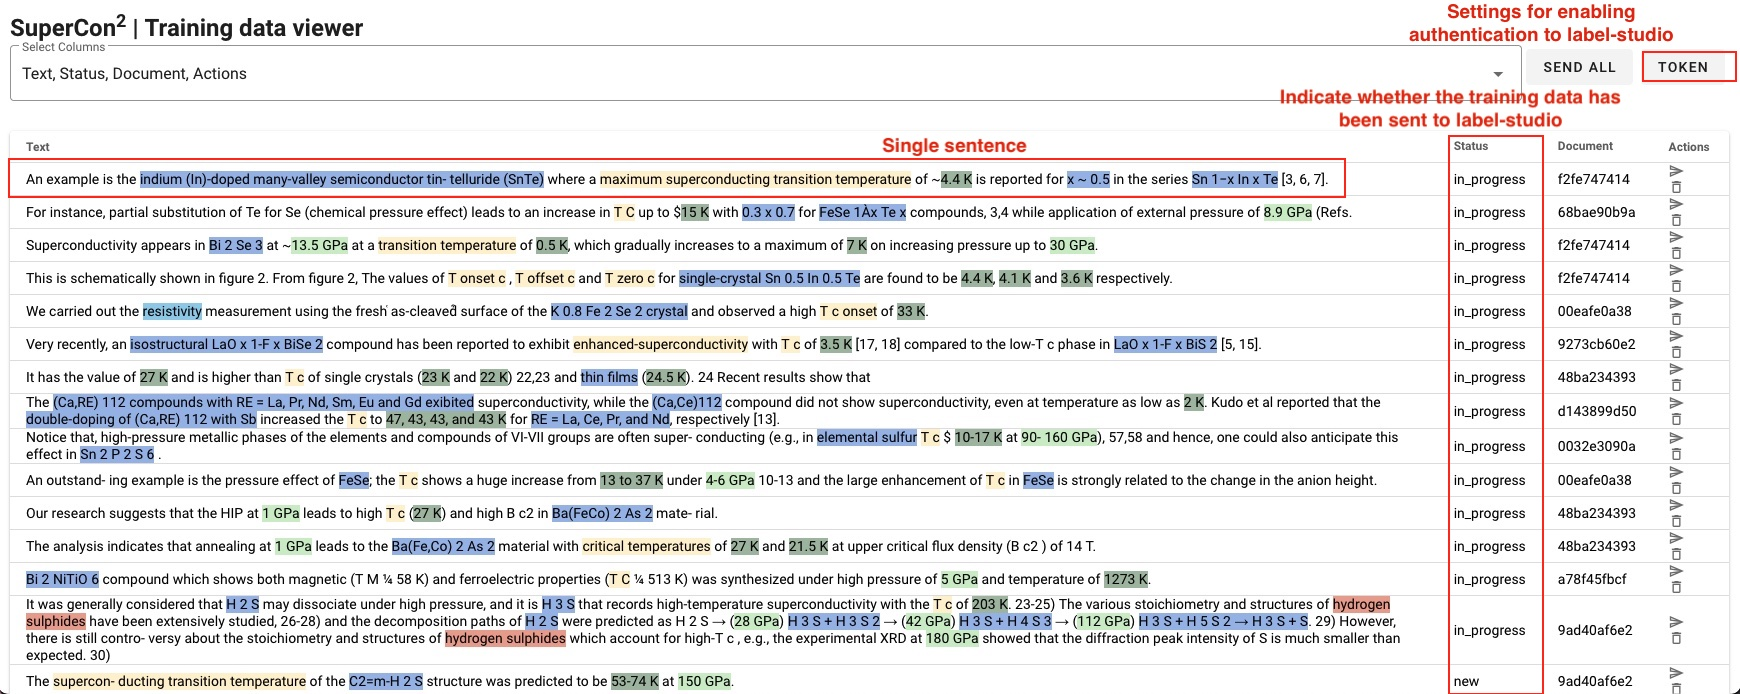
\includegraphics[width=1\textwidth]{images/training-data-viewer} 
  \caption{Training data view}
  \label{fig:training-data-view}
\end{figure}

Since the training data generated with this interface are related to proven mistakes in the TDM process, intuitively they should provide a higher impact in improving the model than training data of the same amount, randomly selected.
To prove this hypothesis, we performed an experiment: we selected around 400 training examples initially marked as incorrect by the anomaly detection script and we curated them. 
Then, we collected the training data and manually correct them, keeping only training data that was actually corrected. 
We obtained 352 examples (curation) which were added to the SuperMat examples (Base). 

In this experiment we focused on the best model which is based on SciBERT, and that can be trained with two different strategies: from scratch (s) or incrementally (i).
We defined three scenario: a) Base from scratch, b) Base+curation from scratch, and c) Base from scratch and then Base+curation incrementally.

[TODO: clarify why do we need Base+curation incrementally??]

The obtained models are tested using a fixed holdout dataset we have designed in our previous work~\cite{lfoppiano2023automatic} and the evaluation scores are illustrated in Table~\ref{tab:evaluation-curation-training}.

\begin{table}[h]
\centering
\begin{tabular}{|l|l|l|l|}
\hline
& \textbf{Base} & \textbf{base+curation(s)} & \textbf{base(s)+curation(i)} \\ 
\hline
\hline
Nb total examples & 16902 & 17254 & 16902(s), 17254 (i)\\ 
\hline
\texttt{<class>}        & 70,22             & 72,30             & \textbf{72,63} \\ 
\texttt{<material>}     & 79,69             & 80,23             & \textbf{80,61} \\ 
\texttt{<me\_method>}   & 64,78             & 65,31             & \textbf{66,62} \\ 
\texttt{<pressure>}     & \textbf{46,96}    & 46,53             & 46,84 \\ 
\texttt{<tc>}           & 77,36             & 78,56             & \textbf{79,57} \\ 
\texttt{<tcValue>}      & 77,26             & \textbf{77,94}    & 77,84 \\ 
\hline
\textbf{All (micro avg.)} & 75,86           & 76,66             & \textbf{77,36} \\ 
\hline
\textbf{Diff avg. w/ baseline}& -           & +0,80             & \textbf{+1,50} \\ 
\hline
\end{tabular}
\caption{Evaluation scores and comparison of fine-tuning training of SciBERT. The Base dataset is the original dataset described in~\cite{lfoppiano2023automatic}, the curation dataset is automatically collected based on the database corrections by the interface and manually corrected. \textit{s} indicate "training from scratch", while \textit{i} indicate "incremental training". The results are the average of 5 repeated train/eval runs. }
\label{tab:evaluation-curation-training}
\end{table}

The result of this experiment is that with only 352 examples (0.002) we obtained an improvement of +1.50\% F1 score. The incremental approach obtained almost twice the improvement of the model trained from scratch with the extended dataset. 
There are several hypothesis for this, one could argue that the dataset is not big enough for the task at hand, therefore the model requires more training time. This issue could be verified by correcting all the avaialble training data and repeat this experiment. 


\section{Code availability}
This application is freely available at \url{https://github.com/lfoppiano/supercon2}, the repository contains:
\begin{itemize}
\item SuperCon 2 curation interface for visualising and editing material and properties extracted from superconductors-related papers.
\item The ingestion workflow to create process PDF documents with grobid-superconductors and produce a database of materials and properties.
\end{itemize}

\section{Conclusions}
We built a staging area for SuperCon where the data automatically extracted can be examined and corrected by curators in an efficient manner. Thanks to visual aid and contextual connections we improve the quality of curators and their throughput, while providing an efficient system for updating the SuperCon database. 
We demonstrated that the feedback loop based on corrected data can improve substantially the machine learning models with fresh and targeted training data. 

There are several planned features and improvements in the pipeline. Some of these include:

\begin{itemize}
    \item Undo/redo functionality: The ability to undo and redo changes made to records will be added, to make it easier to correct mistakes.
    \item Document versioning: A versioning system will be implemented to track changes to documents over time.
    \item Improved search: The search functionality will be improved to make it easier to find records based on specific criteria.
    \item Additional record types: SuperCon 2 currently supports records for material and property information, but additional record types will be added in the future.
\end{itemize}

\bibliography{references}
\bibliographystyle{plain}

\end{document}



